% vim: set fenc=utf-8 ft=latex encoding=utf-8
% -*- mode: latex; coding: UTF-8; -*-
%!TEX root = knowledge-curation.tex
\section{Findings}
\label{cha:findings}
This study focused on how knowledge---in the form of questions and answers---is created, shared, and curated. We first identified and categorized the main types of knowledge contained in the \RH mailing list and in \SO messages with the R tag (RQ1). The emerging categories formed a typology, and allowed us to identify and describe two approaches for constructing knowledge that are supported by these channels (RQ2). Interestingly, we found that some developers are active on both channels, and in some cases, even post the same questions. As a result, we investigated the benefits they gain by doing so (RQ3). In this section, we present our findings.
%This section presents the findings of our study that answer each research question.

\subsection{What Types of Knowledge Are Shared on \SO and the \RH Mailing List}
%\subsection{RQ-1. \rqa}
\label{cha:findings-types}

To answer RQ1, we randomly sampled 400 threads of messages from both \SO and the \RH mailing list, where each thread included a question and the associated responses. We identified five main types of knowledge:
\begin{enumerate*}[label=(\arabic*)]
\item Questions
\item Answers
\item Updates
\item Flags
\item Comments.
\end{enumerate*}
Each of these types is further divided into sub-types. Table~\ref{table:type-of-knowledge} presents the typology of knowledge types, their description, and the frequency in the sample of 400 threads. As mentioned in Section~\ref{cha:methodology}, this sample provides a reliability of 95\% $\pm$ 5\%. Using the Chi-square test of independence, we tested whether the distribution of types and sub-types of questions were different between the two channels.  In
all cases, they were found to be statistically different (with $\rho \ll 0.001$ in all cases).
    \begin{table*}[!htb]
      \centering
      \caption{Typology of knowledge types found on both \SO (SO) and \RH (RH), and their frequency in the analyzed sample. Numbers in bold represent the most significant differences between the two sets.}
      \begin{small}
\begin{tabular}[h]{p{2.3cm}p{10.3cm}rrrrr}
 && \textbf{SO}                                                                                                                                              & \textbf{RH}  & \textbf{Prop SO} & \textbf{Prop RH}                \\
\toprule
\multicolumn{2}{@{}l}{\textbf{Questions}}\\
  \emph{How-to}                   & Asks how to do something specific.                                                                                                                        & {166}          & {103}              & \textbf{41.50\% }       & \textbf{25.75\%}        \\
  \emph{Bug/Error\-/Exception}    & Asks for a solution or reasons for an error message.                                                                                                       & 27           & 48               & 6.75\%         & 12.00\%        \\
  \emph{Discrepancy}              & Asks about an unexpected result of a specific function, process, or package.                                                                              & 53           & 88               & \textbf{13.25\%}        & \textbf{22.00\%}        \\
  \emph{Set-up}                   & Asks for possible ways to set up the R environment before or after deployment.                                                                            & 15           & 31               & 3.75\%         & 7.75\%         \\
  \emph{Decision help}            & Asks for advice in making a decision.                                                                                                                     & 36           & 35               & 9.00\%         & 8.75\%         \\
  \emph{Conceptual\-/Guidance}    & Asks for conceptual clarification or guidance on topics related to R or statistics.                                                         & 48           & 49               & 12.00\%        & 12.25\%        \\
  \emph{Code reviewing}           & Asks for a code review, explicitly or implicitly.                                                                                                           & 34           & 21               & 8.50\%         & 5.25\%         \\
  \emph{Non-functional}           & Asks for help (or suggestions) with a non-functional requirement such as performance or memory usage.                                                   & 14           & 11               & 3.50\%         & 2.75\%         \\
  \emph{Future reference}         & Asks a question (often self-answering it) that might not exist on the channel, but that is interesting enough to warrant a thread for future reference.         & 5            & 4                & 1.25\%         & 1.00\%         \\
  \emph{Other}                    & Asks for assistance unrelated to the channel, or the message contains unrelated information (e.g., announcements, ideas for improvement).                  & 2            & 10               & 0.50\%         & 2.50\%         \\\cline{3-6}
                                  &                                                                                                                                                          & {400} & {400}     & {100\%} & {100\%} \\
\hline
  \multicolumn{2}{@{}l}{\textbf{Answers}}                                                                                                                                                                                                                          \\
  \emph{Redirecting}                & Provides a link to an existing solution that is not in the thread (e.g. external application, tutorial, project).                                     & 163          & 87               & 20.20\%        & 15.03\%        \\
  \emph{Tutorial}                   & Provides a set of steps to teach people how to solve the issue.                                                                                          & 105          & 15               & \textbf{13.01\%}        & \textbf{2.59\% }        \\
  \emph{Source code}                & Provides a source code snippet as the solution without an extensive explanation about the answer.                                                                   & 198          & 102              & 24.54\%        & 17.62\%        \\
  \emph{Clue/Suggestion/Hint}       & Provides a possible way(s) to fix the issue without actually solving it.                                                                                                     & 43           & 105              & \textbf{5.33\% }        & \textbf{18.13\% }       \\
  \emph{Alternative}                & Provides a different approach to a solution that is related to but not exactly what is being asked (e.g. mathematical approach, data structure modification). & 33           & 98               & \textbf{4.09\% }        & \textbf{16.93\% }       \\
  \emph{Explanation}                & Provides an explanation of an approach that answers the question and lists steps on how to do it.                                                                          & 203          & 101              & 25.15\%        & 17.44\%        \\
  \emph{Announcement}               & Provides a notification about some artifact (e.g., packages, libraries).                                                                                 & 8            & 33               & 0.99\%         & 5.70\%         \\
  \emph{Benchmark}                  & Provides a benchmark of multiple solutions posted by others or compares different answers.                                                               & 5            & 3                & 0.62\%         & 0.52\%         \\
  \emph{Opinion}                    & Provides an opinion or an expansion of another answer by including scenarios and examples.                                                                    & 49           & 35               & 6.07\%         & 6.04\%         \\\cline{3-6}
                                    &                                                                                                                                                          & \textbf{807} & \textbf{579}     & {100\%} & {100\%} \\
\hline
  \multicolumn{2}{@{}l}{\textbf{Updates}}                                                                                                                                                                                                                          \\
  \emph{Announcement}               & Announces specific events (e.g., bounties, future updates).                                                                                              & 27           & 3                & 4.40\%         & 1.21\%         \\
  \emph{Background}                 & Adds additional context to the question or answer .                                                                                                       & 74           & 57               & 12.07\%        & 23.08\%        \\
  \emph{Correction}                 & Corrects format, grammar, spelling, and semantic mistakes.                                                                                               & 301          & 2                & \textbf{49.10\% }       & \textbf{0.81\% }        \\
  \emph{Expansion}                  & Expands the question or answer by providing scenarios or examples.                                                                                       & 116          & 83               & \textbf{18.92\% }       & \textbf{33.60\%}        \\
  \emph{Explanation}                & Explains or clarifies a specific point in the question or answer, such as why the user chose a specific data structure, or the meaning of a variable.    & 83           & 95               & 13.54\%        & 38.46\%        \\
  \emph{Solution}                   & The user answers their own question.                                                                                                                     & 12           & 7                & 1.96\%         & 2.83\%         \\\cline{3-6}
                                    &                                                                                                                                                          & \textbf{613} & \textbf{247}     & {100\%} & {100\%} \\
\hline
  \multicolumn{2}{@{}l}{\textbf{Flags}}                                                                                                                                                                                                                            \\
  \emph{Off-topic/Opinion}          & Identifies questions that are unrelated to the channels' interests or which answers seek opinion.                                                      & 22           & 19               & 27.16\%        & 35.19\%        \\
  \emph{Not an answer}              & Emphasizes \textit{alternative answers} out of the scope of the question, or identifies that a solution does not answer the question.                    & 0            & 27               & \textbf{0.00\% }        & \textbf{50.00\%}        \\
  \emph{Repeated question}          & Notifies a user that the question has been answered previously.                                                                                                & 48           & 8                & \textbf{59.26\%}        & \textbf{14.81\%}        \\
  \emph{Too localized}              & Questions that are too specific and might not help future readers.                                                                                    & 6            & 0                & 7.41\%         & 0.00\%         \\
  \emph{Unclear}                    & Questions that are difficult to understand.                                                                                                              & 5            & 0                & 6.17\%         & 0.00\%         \\\cline{3-6}
                                    &                                                                                                                                                          & {81}  & {54}      & {100\%} & {100\%} \\
\hline
  \multicolumn{2}{@{}l}{\textbf{Comments}}                                                                                                                                                                                                                     \\
  \emph{Clarification}          & Provides (or requests) additional information about a question or answer.                                                                                & 98           & 28               & 17.44\%        & 10.49\%        \\
  \emph{Expansion}              & Provides additional information.                                                                                                                         & 127          & 65               & 22.60\%        & 24.34\%        \\
  \emph{Correction/Alternative} & Suggests a change to a question or answer, offers an alternative solution or a correction.                                                               & 102          & 89               & \textbf{18.15\%}        & \textbf{33.33\% }       \\
  \emph{Compliment/Critic}   & Posts something good, offers thanks, provides an opinion or criticism.                                                                           & 157          & 52               & 27.94\%        & 19.48\%        \\
  \emph{External reference}     & References an external resource.                                                                                                                         & 78           & 33               & 13.88\%        & 12.36\%        \\\cline{3-6}
                                &                                                                                                                                                          &{562}  & {267}     & {100\%} & {100\%} \\
  \bottomrule
        \end{tabular}
      \end{small}
      \label{table:type-of-knowledge}
\vspace{-3mm}
    \end{table*}

\paragraph*{Questions and Answers}
    Questions express one or more problems or concerns faced by a user on the \RH mailing list or \SO, whereas answers represent solutions to questions.  We observed that the types of questions on \SO are more specific than those on the \RH mailing list and in \SO answers are more likely to be tutorials. Also, \SO has more answers per question---2 per question compared to 1.4 for \RH. However, \RH answers tend to offer more suggestions or alternatives than \SO answers. %This might be a result of the narrowness of \SO questions.

\paragraph*{Updates}
An update is a modification of a question or answer. In \SO, updates are presented in one of two ways:
\begin{description}[itemsep=3pt, topsep=2pt, leftmargin=1em, parsep=0pt]
\item[Labeled updates] are explicitly shown in the body of questions or answers next to a label that identifies the update (e.g., edit, update, and p.s.).
  When multiple update labels appear in a message, each label is accompanied by a number (e.g., \textit{``[Edit 1:]''}), a date (e.g., \textit{``Edit/Update (April 2011):''}), or a bulleted list
  (e.g., ``EDIT: - anova... -drop1...'').

\item[Non-labeled updates] are only visually recognizable through the message history system. The only indication of the change is a box at the end of the
  message that contains the user who performed the change and the date when it happened.
\end{description}
We found that \textit{Non-labeled} updates are often used to correct formatting, grammar, semantic mistakes, and spelling, or to incorporate explanations, examples, and suggestions without changing the meaning of the question or answer. \textit{Labeled} updates are for everything else.

In \RH, all communication is done through emails, and authors do not explicitly tag them as updates. For this reason, we define an update on \RH as \emph{a message sent to a thread where the author has already participated once}.

Regarding update frequency in our sample, the \SO R tag contained 2.5 more updates than the \RH mailing list. Corrections are more common in \SO (almost 50\%), while \RH updates are often related to the adding of information to a thread (providing background, expansion, and explanation).

\paragraph*{Flags}
Flags are used to alert members of the community.

\SO contains a flagging mechanism, often used to get a moderator's attention. These flags can accomplish various objectives: mark a message as containing spam, rude, or abusive behavior; or identify
duplicate questions, off-topic messages, unclear questions, opinion-based questions, and low-quality
answers. Depending on the type of flag, this can lead to a thread being closed or the loss of user reputation points.  

\RH doesn't have a built-in flagging mechanism, however, \RH users utilize the concept of flags, which we define as \emph{messages used to call the attention of other community members}, similar to how flags are used in \SO.

% The main objective of Flags in both channels is to 
% keep a
% healthy community, promote discussion, and to raise specific
% issues.  %Flags we found in emails that also contained other types of information (such as answers, comments, and updates).

% Hance, flags in the \RH mailing list do not constrain users to answer questions, or to clarify
% what it is already asked.
% Under our definition, flags might be used by the person who asked or answered a question
% (in \SO authors of a question cannot add flags to it). 

In terms of their frequency, R tag posts on \SO had 1.5 times more flags than posts on the \RH mailing list. \SO flags are primarily used to mark repeated questions. In contrast, flags on \RH are often used to indicate that a previous answer is incorrect.

\paragraph*{Comments}

In \SO, comments are considered ``temporary `Post-It' notes left on a question or answer''\footnote{\url{http://stackoverflow.com/help/privileges/comment}}. Comments are located below each question or answer and can be used as a follow-up to a question, or to answer or clarify a question. In \RH, we define comments as messages written to \emph{improve an answer or as a follow-up to a discussion}. It should be noted that in order for an email to qualify as a comment, it should not be written by the person who asked or answered the original question (otherwise, the message would be considered an update).
Because both \SO and \RH permit participants to ask multiple questions in the same thread, the sub-categories of comments are not mutually exclusive.  

Regarding the frequency of comments, the main difference between both channels is that \SO comments are less likely to be considered corrections or alternatives (Correction/Alternative sub-category) than in \RH. The \SO R tag sample also contained 2.1 times more comments than the \RH sample.

\subsection{How Is Knowledge Constructed on \SO and the \RH Mailing List}
%\subsection{RQ-2. How is knowledge constructed on \SO and the \RH mailing list?}
\label{sec:rq2}

Our analysis helped us identify two different approaches used for constructing knowledge (RQ2) on \SO and the \RH Mailing List: participatory knowledge construction and crowd knowledge construction.

\begin{description}[itemsep=2pt, topsep=0pt, leftmargin=1em, parsep=0pt]
\item[Participatory knowledge construction] is an approach where answers are created through the cooperation of multiple users in the same thread. Participants complement each other's questions by discussing the pros and
  cons of each answer, and by adding different viewpoints, additional information, and examples.
  This process is similar to a team working together towards
  a common objective.

\item[Crowd knowledge construction] leverages the experiences of many users who work in a relatively
  independent manner. Each user contributes to the thread, adding variety to the pool of solutions. However, the user's priority is to provide a correct answer and not to discuss other solutions.
  This is comparable with the concept of a group in which people work towards the same objective but not necessarily together (e.g., Amazon's Mechanical Turk). Participants can vote on other's ideas, but the
  main idea is not constructed through a discussion process.
\end{description}

In the \RH mailing list, \textit{participatory knowledge} construction takes place when:
\begin{enumerate*}[label=(\arabic*)]
  \item previous answers are included in the current answer with clear links between them; or
  \item a reply contains a direct reference to other answers or authors.
\end{enumerate*}
Figure \ref{fig:ML-PK1} depicts two examples of the way participatory knowledge occurs on the \RH mailing list: direct citation of the author of a previous answer, and inferable links between answers.

    
    \begin{figure}[!htb]
        \centering
        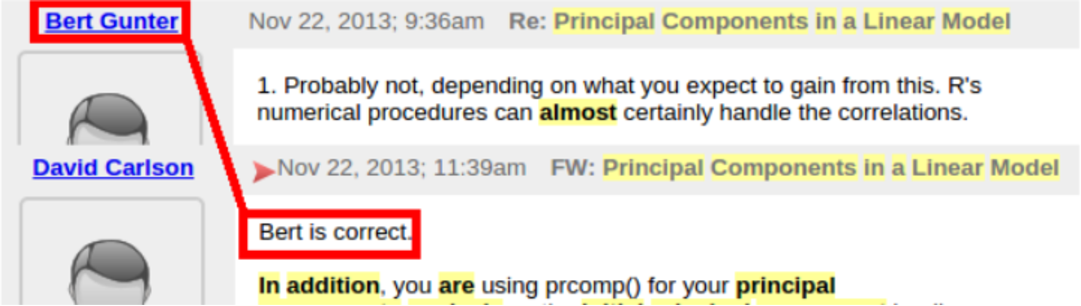
\includegraphics[width=\columnwidth]{Figures/ML-PKimg2}
        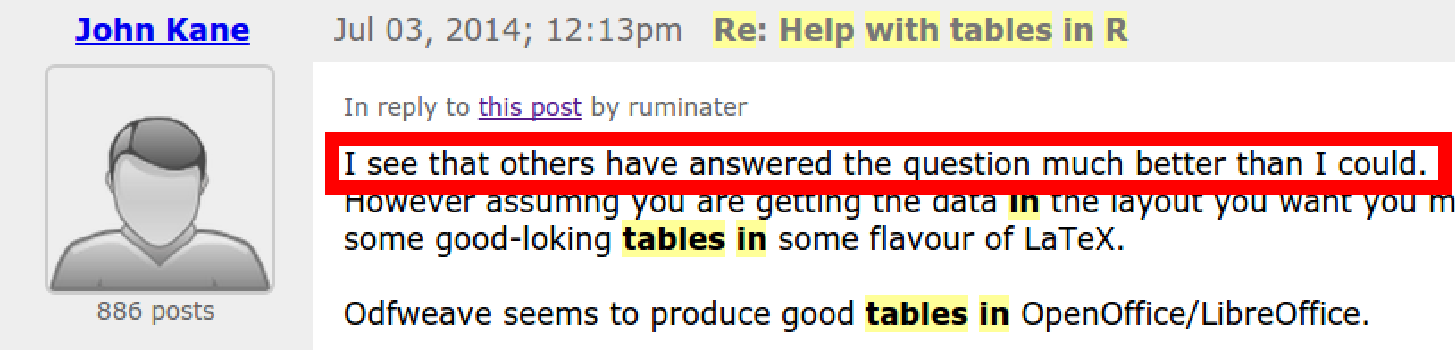
\includegraphics[width=\columnwidth]{Figures/ML-PKimg11}
        \caption[Participatory knowledge construction on the \RH mailing list.]{Participatory knowledge construction on the \RH mailing list.}
        \label{fig:ML-PK1}
      \vspace{-3mm}
    \end{figure}

In \SO, \textit{participatory knowledge} construction takes place when:
    \begin{enumerate*}[label=(\arabic*)]
    \item one can infer a link between answers, through either a direct or indirect reference; or
    \item comments complement the answer or directly cite another author.
    \end{enumerate*}
Participatory knowledge construction also occurs in different places on \SO, perhaps as a consequence of its rich interface. We observe this type of knowledge construction when a user answers a question and directly cites or links to someone else's answer in the thread, or when a user cites someone else's question or answer in a comment (a typical case is linking to a previously asked question). Figure \ref{fig:SO-PK1} depicts an example of participatory knowledge construction on \SO: a user added a comment to help another user when the answer was not sufficient, and---in the comment---they referenced another author's answer.

    \begin{figure}[!htb]
        \centering
        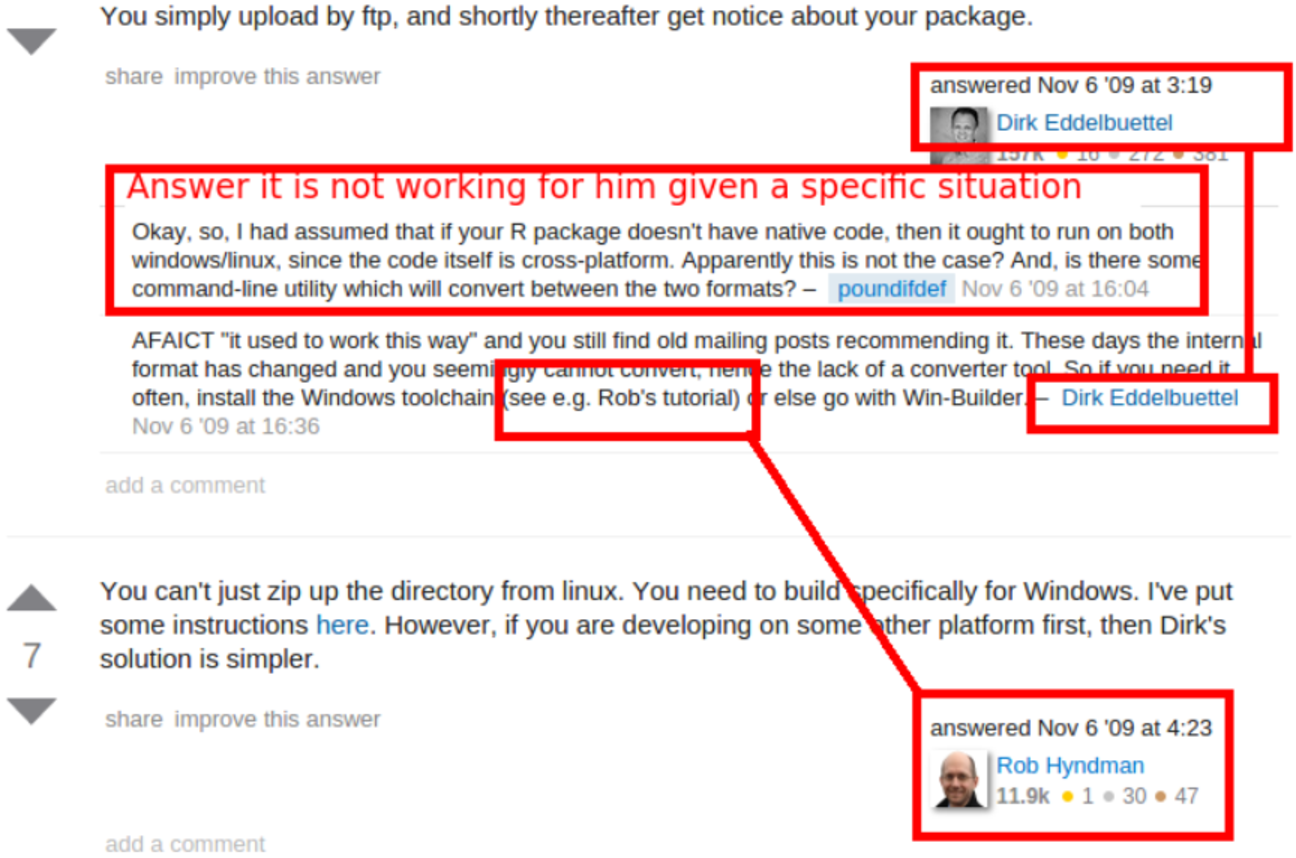
\includegraphics[width=\columnwidth]{Figures/SO-PKimg5}
        \caption{Example of participatory knowledge on \SO. Users build on the comments and answers of other users.}
        \label{fig:SO-PK1}
        \vspace{-3mm}
    \end{figure}

In \SO \textit{Crowd knowledge} construction is observable when
  \begin{enumerate*}[label=(\arabic*)]
    \item there is no direct or inferable reference between answers; or
    \item an answer is a variation of one of the other answers on the thread.
  \end{enumerate*}
Figure \ref{fig:CKC_MLSO} depicts an example of crowd knowledge construction on \SO. As can be seen from the figure, two of the three answers provided the same solution. 

In the \RH mailing list, we observed \textit{Crowd knowledge} construction when different messages were responding directly to the original question (rather than responding to a response).

    \begin{figure} [!htb]
        \centering
        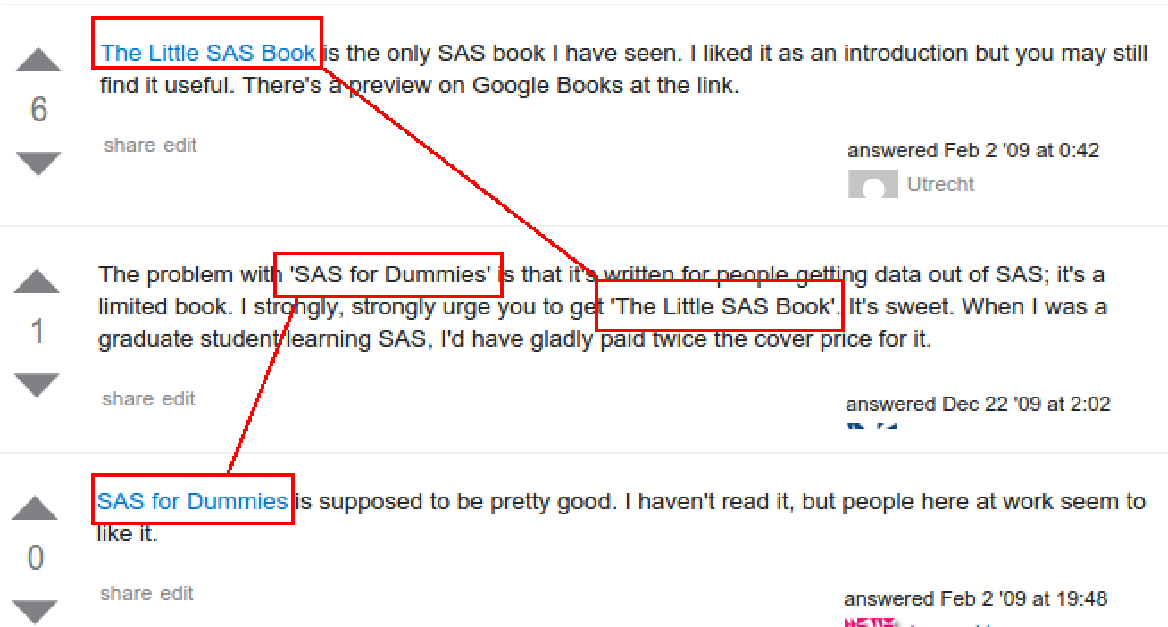
\includegraphics[width=\columnwidth]{Figures/SO-CSimg2}
        \caption{Example of how crowd knowledge construction occurs. The three authors provide similar answers, but they do it independently of each other.}
        \label{fig:CKC_MLSO}
\vspace{-3mm}
    \end{figure}

\subsection{Why Users Post to a Particular Channel}
%\subsection{RQ-3. Why do certain users post to both \SO and the \RH mailing list}
Some survey participants stated their preference of one channel over the other. We summarize their responses below.

\subsubsection{Why Participants Post on \SO}

Survey participants preferred using \SO for several reasons: (a) the ability to gain peer recognition (the advantage of gaining points---and visibility---is a major draw of \SO); (b) its rich and user-friendly interface; (c) answers are straight to the point; (d) questions are usually answered faster on \SO than \RH; and (e) it is easy to search for previous questions and answers.

However, the respondents reported a few main drawbacks of using \SO: (a) there is an overabundance of related questions; (b) one requires a certain level of experience to understand some of the answers; and (c) \SO's strict rules only allow questions and their answers, they do not allow discussions nor questions about opinions.


\subsubsection{Why Participants Post on \RH}
\label{sec:rh}

Survey participants reported a few benefits of using the \RH mailing list: (a) the email format is convenient; (b) following the mailing list provides awareness and increases learning in new topics; (c) there is more flexibility regarding the topics that one can discuss; and (d) there is a lot of participation from highly experienced users. The respondents did note a couple of disadvantages of \RH: (a) some discussions lead to aggressive behavior; and (b) searching the archives is not easy.

\subsubsection{Why Participants Post to Both Channels}

Our analysis of the archived data revealed that some users (79 cases in our sample) posted the same question on both channels. 
%The survey provided deeper insights on why R members act this way.
Based on the responses from the survey, we identified that being active on both channels brings benefits to those asking and answering questions (RQ3):

\begin{description}[itemsep=2pt, topsep=0pt, leftmargin=1em, parsep=0pt]
\item[Find a better answer:] As expected, two channels are better than one as 
  one channel might result in a better answer than the other.
\item[Support follow-up questions:] We found that \RH is often used to conduct follow-up discussions on
  specific answers provided to \SO questions. \SO's focus is on finding an answer to a question and does not
  provide an environment to discuss the specifics of an answer (unless it is asked as another question).
In contrast, a discussion on \RH can continue long after an answer has been found through follow-up questions, and not only by the person who asked the original question.  
\item[Speed up answers:] Members ask the same question on both channels in order to get an answer faster. However, this behavior is not encouraged by the community as it is deemed impolite\footnote{\href{https://goo.gl/p9vVaj}{https://goo.gl/p9vVaj}}.
% `... it's impolite to cross post across several lists (i.e., \SO and \RH)''
\end{description}





%%% Local Variables:
%%% mode: latex
%%% TeX-master: "knowledge-curation.tex"
%%% End:
